%---------------------------------------------------------------------
%                          Capítulo 4
%---------------------------------------------------------------------
\chapter{Aspectos operativos}
\section{Cronograma}
El cronograma planteado se puede ver en la figura \ref{fig:cronograma}
\begin{figure}[h]
    \centering
    \captionsetup{justification=centering}
    %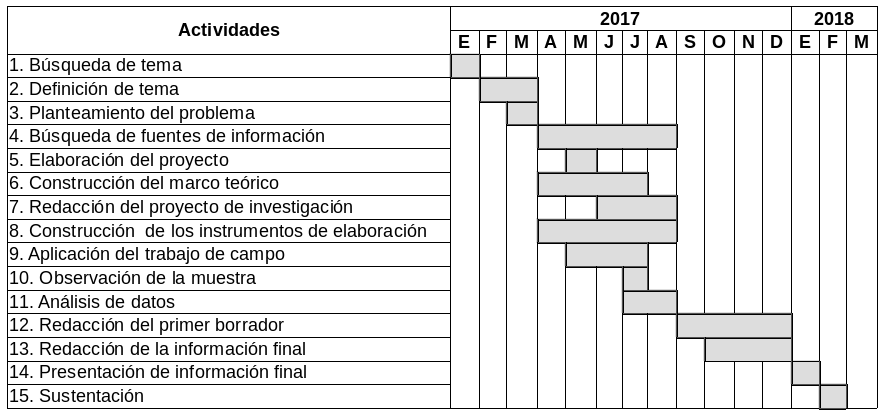
\includegraphics[width=1.0\textwidth]{Imagenes/Bitmap/cronograma}
    %----

    \begin{ganttchart}[
      hgrid=true,
      vgrid={*{11}{black, dotted},*1{black},*3{black, dotted}},
      x unit=0.7cm,
            y unit title=0.7cm,
            y unit chart=0.8cm,
            bar label node/.style={text width=4cm,align=left,font=\scriptsize\RaggedLeft,anchor=east},
    ]{1}{16}
      \ganttset{bar height=.6}
      \ganttset{bar/.append style={fill=lightgray}}
      \gantttitle{2017}{12}
      \gantttitle{2018}{4} \\
      \gantttitlelist{1,...,12,1,2,3,4}{1} \\

      \ganttbar{Búsqueda de tema}{1}{1} \\
      \ganttbar{Definición de tema}{2}{3} \\
      \ganttbar{Planteamiento del problema}{4}{4} \\
      \ganttbar{Búsqueda de fuentes de información}{5}{8} \\
      \ganttbar{Elaboración del proyecto}{5}{5} \\
      \ganttbar{Construcción de marco teórico}{4}{7} \\
      \ganttbar{Redacción del proyecto de investigación}{6}{8} \\
      \ganttbar{Construcción de los instrumentos de investigación}{4}{8} \\
      \ganttbar{Aplicación del trabajo de campo}{5}{7} \\
      \ganttbar{Observación de la muestra}{7}{7} \\
      \ganttbar{Análisis de datos}{7}{8} \\
      \ganttbar{Redacción del primer borrador}{9}{12} \\
      \ganttbar{Redacción del informe final}{10}{12} \\
      \ganttbar{Presentación del informe final}{14}{15} \\
      \ganttbar{Sustentación}{16}{16}
    \end{ganttchart}
    %----
    \caption{Cronograma de trabajo}
    \label{fig:cronograma}
\end{figure}

\section{Presupuesto y financiamiento}
El presupuesto para la realización se puede ver en la tabla \ref{t:presupuesto}.
El financiamiento será asumido integramente por el tesista.

\begin{table}[]
  \centering

  \begin{tabular}{|p{5cm}|p{3cm}|p{3cm}|}
    \hline
    \thead{Detalle} & \thead{Prec. Unit.} & \thead{Sub Total} \\ \hline
    Material de escritorio &  &  \multicolumn{1}{r|}{400.00} \\ \hline
    Anillados & \multicolumn{1}{r|}{5.00}  &  \multicolumn{1}{r|}{45.00} \\ \hline
    Copias &  &  \multicolumn{1}{r|}{90.00} \\ \hline
    Adquisición de bibliografia  &  & \multicolumn{1}{r|}{400.00} \\ \hline
    Empastados &  \multicolumn{1}{r|}{30.00}  & \multicolumn{1}{r|}{90.00} \\ \hline
    Transporte &    & \multicolumn{1}{r|}{100.00} \\ \hline
    Corrector de estilo &    & \multicolumn{1}{r|}{300.00} \\ \hline
    Asesor estadístico &    & \multicolumn{1}{r|}{300.00} \\ \hline
    Servicios (Internet) & \multicolumn{1}{r|}{80.00} & \multicolumn{1}{r|}{240.00} \\ \hline
    Elaboración de software   &  & \multicolumn{1}{r|}{23 100.00} \\ \hline
    Aplicación de instrumentos  & \multicolumn{1}{r|}{300.00} & \multicolumn{1}{r|}{300.00} \\ \hline
    \textbf{TOTAL}  &  & \multicolumn{1}{r|}{25 665.00} \\ \hline
  \end{tabular}
  \caption{Presupuesto}
  \label{t:presupuesto}
\end{table}

\section{Matriz de consistencia}
La matriz de consistencia de este trabajo se muestran en las tablas \ref{t:consistencia}
y \ref{t:consistencia_cont}.

\begin{sidewaystable}[htbp]
\centering
\caption{Matriz de consistencia}
\label{t:consistencia}
\begin{tabular}{|p{5cm}|p{6cm}|p{6cm}|p{4cm}|}
\hline
\thead{Problema} & \thead{Objetivo} & \thead{Hipotesis} & \thead{Variables} \\ \hline
\textbf{Problema general}

¿Cual es el efecto del uso de las herramientas de la computación en la nube
en la gestión de las MiPYME pertenecientes al Centro de Desarrollo Empresarial
del Cusco?.

\textbf{Problemas específicos}

\begin{enumerate}[noitemsep]
\item Cuál es el nivel de gestión de las MiPYMES pertenecientes al Centro
de Desarrollo Empresarial del Cusco antes del uso de herramientas de la computación
en la nube.
\item Cuál es el nivel de gestión de las MiPYMES pertenecientes al Centro
de Desarrollo Empresarial del Cusco después del uso de herramientas de la computación
en la nube.
\end{enumerate}
&
\textbf{Objetivo general}

Determinar el efecto del uso de la computación en la nube en la gestión de
las micro, pequeñas y medianas empresas pertenecientes al Centro de desarrollo
empresarial del Cusco.

\textbf{Objetivos específicos}
\begin{enumerate}
  \item Determinar el nivel de gestión de las MiPYMES pertenecientes al Centro de
  Desarrollo Empresarial del Cusco antes del uso de las herramientas de la
  computación en la nube.
  \item Determinar el nivel de gestión de las MiPYMES pertenecientes al Centro de
  Desarrollo Empresarial del Cusco después del uso de las herramientas de la
  computación en la nube.
\end{enumerate}
&
\textbf{Hipótesis general}

Existe un efecto positivo del uso de la computación en la nube en la
gesti'on de las micro, pequeñas y medianas empresas pertenecientes al Centro de
Desarrollo Empresarial del Cusco.

\textbf{Hipótesis específicas}
\begin{enumerate}[noitemsep]
    % preguntaar si es necesario colocar las palabras pe-post implementacion
    \item El nivel de gestión de las MiPYMES pertenecientes al Centro de Desarrollo
          Empresarial del Cusco antes del uso de las herramientas de la computación
          en la nube es deficiente.
    \item El nivel de gestión de las MiPYMES pertenecientes al Centro de Desarrollo
          Empresarial del Cusco después del uso de las herramientas de la computación
          en la nube es eficiente.
    \item El efecto del uso de herramientas de la computaci'on en la nube en la
          gestión de las MiPYMES pertenecientes al Centro de Desarrollo Empresarial
          del Cusco es positiva.
\end{enumerate}
&
La única variable identificada es \textbf{Gestión empresarial}.
\\ \hline
\end{tabular}
\end{sidewaystable}

\begin{sidewaystable}[htbp]
\centering
\caption{Matriz de consistencia}
\label{t:consistencia_cont}
\begin{tabular}{|p{7cm}|p{6cm}|p{6cm}|}
\hline
\thead{Justificación} & \thead{Método} & \thead{Universo, población y muestra} \\ \hline
\textbf{Conveniencia}

Conocer el efecto del uso de las herramientas de la computación en la nube en
la gestión de las MiPYME pertenecientes al Centro de Desarrollo Empresarial del Cusco y de esta forma
generar herramientas de apoyo a la gestión lo que permitira lograr su crecimiento.

\textbf{Relevancia social}

Al realizar este estudio se implementaran e implantaran
herramientas de computación en la nube que permitiran mejorar los procesos de gestión
más importantes a un costo razonable que les permita desarrollarse y crecer.

\textbf{Implicancias pr'acticas}

Las herramientas que se implementaran en el presente trabajo mejorarán los procesos
de gestión de las MiPYMEs pertenecientes al Centro de Desarrollo Empresarial del Cusco.

&
\textbf{Enfoque de investigación}

El enfoque para este trabajo será \emph{\textbf{cuantitativo}}.

\textbf{Alcance de investigación}

El estudio que se realizará en el Centro de Desarrollo Empresarial del Cusco será
de \emph{\textbf{alcance explicativo}.}

\textbf{Disenño de investigación}

Debido a que el enfoque para este trabajo es cuantitativo, se deberá realizar
una \emph{\textbf{investigación experimental}} siendo el tipo específico la
\emph{\textbf{preexperimental}}.
&
\textbf{Población y Muestra}

Empresas que son beneficiarias del Centro de Desarrollo Empresarial del Cusco.

\textbf{Tecnicas e instrumentos}

Las técnicas que se aplicarán para este trabajo serán:
la \emph{\textbf{investigación documental}} e \emph{\textbf{investigación de campo}}
utilizando como instrumentos especificos las \emph{\textbf{fichas de trabajo}} y
\emph{\textbf{encuestas}}.

\textbf{Método estadisticos}

Para el análisis de datos se utilizará la \emph{\textbf{Prueba T de Student, Prueba
T-Student o Test-T}}, ya que es la que más se adecua a nuestro escenario.

\\ \hline
\end{tabular}%
\end{sidewaystable}

\section{Matriz de instrumentos}

La matriz de instrumentos de este trabajo se muestran en la tabla \ref{t:instrumentos}

\begin{sidewaystable}[htbp]
  \fontsize{11}{11}
\centering
\caption{Matriz de instrumentos}
\label{t:instrumentos}
\begin{tabular}{|p{2.3cm}|p{4cm}|p{4cm}|p{3cm}|p{3cm}|p{3cm}|}
\hline
\thead{Variable} & \thead{Dimensiones} & \thead{Indicadores} & \thead{Items o reactivos} & \thead{Escala valorativa} & \thead{Instrumentos} \\ \hline
\multirow{10}{3cm}{Gestión empresarial} & \multirow{3}{4cm}{Producción (funciones de seguridad y tecnicas)} & Productividad &  &  & Ficha de trabajo \\ \cline{3-6}
 &  & Eficacia &  &  & Ficha de trabajo \\ \cline{3-6}
 &  & Eficiencia &  &  & Ficha de trabajo \\ \cline{2-6}
 & \multirow{4}{4cm}{Comercialización (función comercial)} & Inventario &  &  & Ficha de trabajo \\ \cline{3-6}
 &  & Ventas &  &  & Ficha de trabajo \\ \cline{3-6}
 &  & Cobranzas &  &  & Ficha de trabajo \\ \cline{3-6}
 &  & Relación con clientes &  &  & Encuensta \\ \cline{2-6}
 & \multirow{3}{4cm}{Administración (funciones contables y financieras)} & Liquidez &  &  & Ficha de trabajo \\ \cline{3-6}
 &  & Endeudamiento &  &  & Ficha de trabajo \\ \cline{3-6}
 &  & Estados financieros &  &  & Ficha de trabajo \\ \hline
\end{tabular}
\end{sidewaystable}

\section{Instrumentos de recolección de datos}
